


\frame
{
  \frametitle{Misura di costanti fisiche fondamentali}

  \begin{itemize}
    \item Misura di e (carica elettrone), h (costante di Planck), k (costante di Boltzmann)
    \item Occasione per affrontare fit complessi (sfruttando tutto quello che state imparando su Likelihood e Chi-Square fits)
    \item Bonus: automazione di acquisizione dati in semplici esperimenti, lavoro di gruppo.        
  \end{itemize}
}

\frame
{
  \frametitle{Misura di costanti fisiche fondamentali}

  \begin{itemize}
  \item Organizzazione in gruppi
    \begin{itemize}
    \item misura di $e/h$ (caratterizzazione caratterizzazione di LED - 2 gruppi)
    \item misura di $e/k$ (caratterizzazione di un transistor - 1 gruppo)
    \item misura di $h/k$ (corpo nero  - 2 gruppi)
    \end{itemize}
  \item Nel pomeriggio di laboratorio: presa dati, comprensione dei risultati, abbozzo analisi dati.
  \item Compito a casa:
    \begin{itemize}
      \item messa punto dell'analisi dati del proprio esperimento e condivisione dei risultati (su aulaweb)
      \item analisi dei dati esperimento Millikan (da cui si ricava $e$)
      \item fit combinato (con tutti i dati del giorno) per estrarre $e$, $h$, $k$. Si minimizza:
        {\footnotesize
    \begin{align*}
      \chi^2 &= {\left( e/h - (e/h)_{meas} \over \sigma(e/h) \right)^2} 
                + {\left( h/k - (h/k)_{meas} \over \sigma(h/k) \right)^2} \\
             &  + {\left( e/k - (e/k)_{meas} \over \sigma(e/k) \right)^2} 
                + {\left(e - (e)_{meas} \over \sigma(e)\right)^2}
    \end{align*}
    }
    \end{itemize}
  \end{itemize}
}

\frame
    {
      \frametitle{Conduttori, semiconduttori, isolanti}

      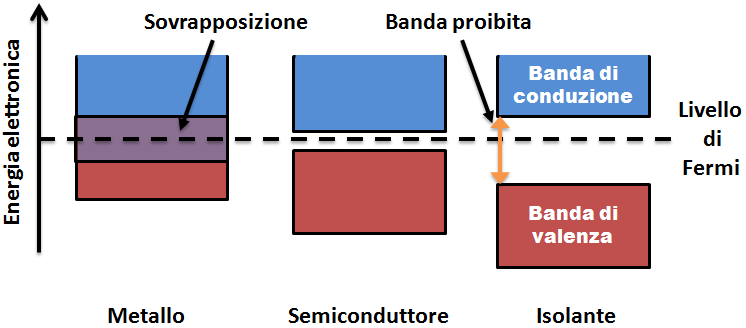
\includegraphics[width=1.0\linewidth]{figs/Stru.png}

    }

\frame
    {
      \frametitle{Semiconduttori p, n. Giunzione p-n}

      \only<1>{
        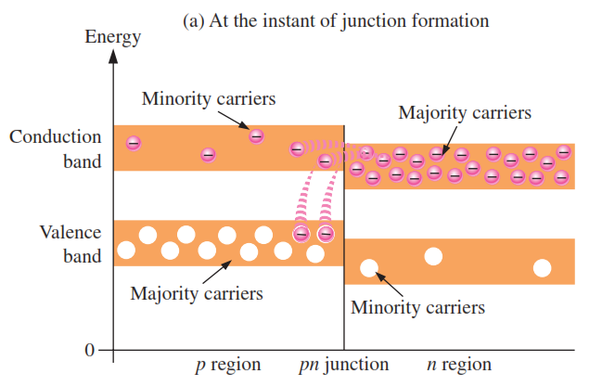
\includegraphics[width=1.0\linewidth]{figs/pn1.png}
      }
      \only<2>{
        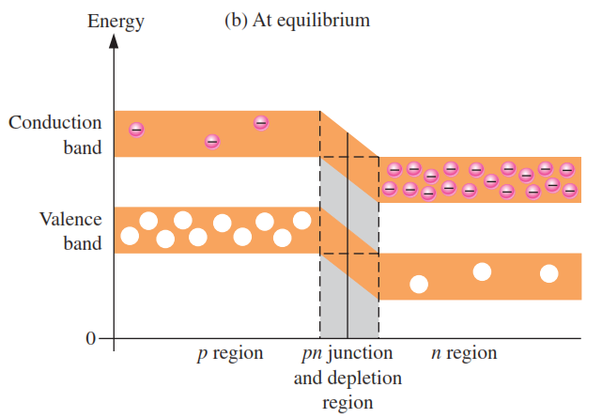
\includegraphics[width=1.0\linewidth]{figs/pn2.png}
      }
    }

\frame    
{
  \frametitle{Misura di $e/h$ tramite curva I-V di un Led}
  
  I LED sono prodotti dalla giunzione di due materiali semiconduttori ``drogati'', uno dei quali ha un eccesso di elettroni (tipo n) e l'altro
  una mancanza di elettroni - indicati anche come fori (tipo p). Quando una corrente elettrica viene iniettata attraverso questa cosiddetta
  giunzione 'p-n', la ricombinazione di elettroni e buchi rilascia energia sotto forma di fotoni.

  \begin{minipage}{0.5\linewidth}{
  \begin{center}
    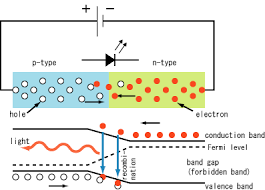
\includegraphics[width=0.9\linewidth]{figs/led.png}
  \end{center}
  }\end{minipage}\begin{minipage}{0.5\linewidth}{
  L'energia dei fotoni emessi ($h\nu$) \`e fornita dal lavoro fatto dal campo elettrico applicato alla giunzione
  ($eV_d$, dove $V_d$ \`e la tensione diretta applicata al diodo) e quindi ci deve essere una relazione lineare:
  \begin{align*}
     h\nu = eV_d + cost
  \end{align*}
  }\end{minipage}
}

\frame
{
  \frametitle{Curva I-V di un Led}

  \begin{minipage}{0.5\linewidth}{
      Di solito si assume per $V_d$ il valore al quale si osserva un "ginocchio" nel punto in cui il diodo comincia a condurre in maniera "apprezzabile".
\vskip 0.1cm
      Questo ``ginocchio'' \`e difficile da misurare
  perch\'e varia significativamente con la scelta della parte della caratteristica che si interpola linearmente.
%    \includegraphics[width=0.8\linewidth]{Led1.pdf}
  }\end{minipage}\hfill\begin{minipage}{0.45\linewidth}{
    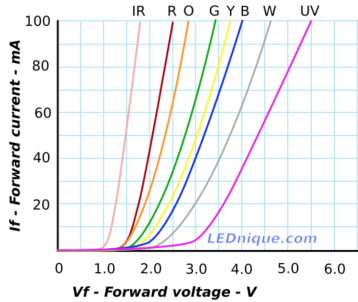
\includegraphics[width=0.8\linewidth]{figs/LedIV.png}
  }\end{minipage}
  \vskip 0.1cm

  Un modo alternativo consiste nel misurare la tensione per cui diversi led conducono la stessa corrente.
  \vskip 0.1cm
  In generale non \`e molto importante misurare $V_d$ quanto una tensione $V^{\prime}$ che differisca da $V_d$ per una costante data
  (potete provare altri approcci).
  \vskip 0.1cm
  Acquisendo la curva I-V per LED di diversi colori si pu\`o fittare la relazione
  \begin{align*}
      V^{\prime} = {e\over h} \nu + cost.
  \end{align*}


}

\frame
{
  \frametitle{Due versioni per la caratterizzazione dei LED}
  \begin{itemize}
  \item misura diretta $I$-$V$ o solo $V$ (assumendo la tensione fornita dal generatore) (gruppo 1)
    \begin{tabular}{cc}
    \includegraphics[width=0.3\linewidth]{figs/Led1.pdf} &
    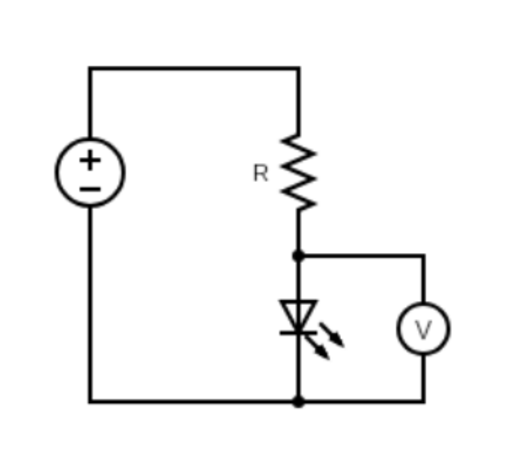
\includegraphics[width=0.3\linewidth]{figs/Led2.pdf}
    \end{tabular}
  \item misura indiretta tramite tensione residua dopo la scarica di condensatore        (gruppo 2)
    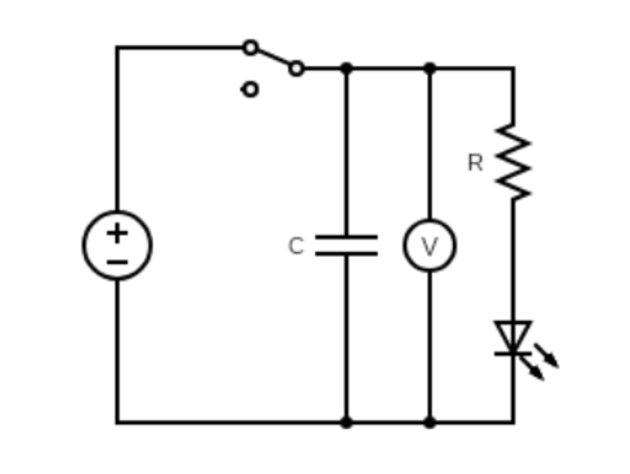
\includegraphics[width=0.3\linewidth]{figs/Led3.pdf}
  \end{itemize}

}

\frame{
  \frametitle{$e/k$ dalla curva IV di un transistor}

  Abbiamo visto che il LED come una particolare giunzione pn (che emette nel visibile: le normali giunzione $pn$ emettono invece nell'infrarosso).
  Quando la giunzione viene creata si instaura una corrente
  \begin{align*}
     I = Ae^{-eV_0\over k T}
  \end{align*}
  che, in assenza di tensione, esterna va a zero. Se si instaura una tensione V che mantiene la giunzione $p$ ad un potenziale positivo
  ed la giunzione $n$ ad un potenziale negativo si instaura una corrente

  \only<1>{
  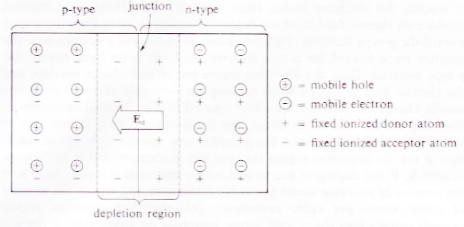
\includegraphics[height=0.3\linewidth]{figs/Jun0.png}
  }
  \only<2>{
  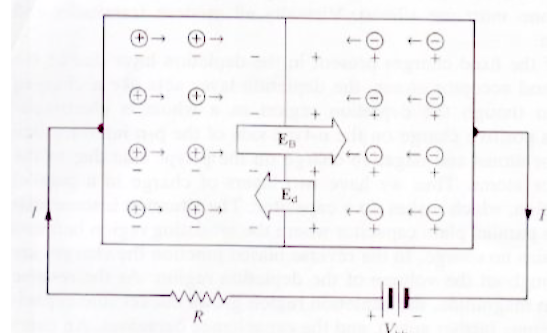
\includegraphics[height=0.3\linewidth]{figs/Jun.png}
  }
}

\frame{
  \frametitle{$e/k$ dalla curva IV di un transistor}

  La corrente totale \`e data da:
  \begin{align*}
     I = Ae^{-e(V_0-V)\over k T} - Ae^{-eV_0\over k T} = Ae^{-eV_0\over kT}\left(e^{eV\over kT} -1\right) = I_0\left(e^{eV\over kT} -1\right)
  \end{align*}
  Tuttavia fattori di non idealit\`a modificano l'equazione in
  \begin{align*}
    I = I_0\left(e^{eV\over \eta kT} -1\right)
  \end{align*}
  dove $\eta$ \`e un parametro che varia da giunzione a giunzione.
}

\frame{
  \frametitle{$e/k$ dalla curva IV di un transistor}
\footnotesize
  Fortunatamente se si considerano due giunzioni ed in particolare un transistor in cui i semiconduttori
  sono disposti nella seguenza $npn$ (emettitore, base e collettore) e  se si mantengono emettitore e base
  sono mantenuti allo stesso potenziale allora la corrente \`e descritta in maniera piuttosto precisa
  con $\eta=1$
  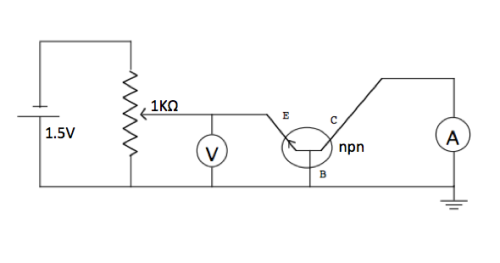
\includegraphics[width=0.6\linewidth]{figs/npn.png}
  \vskip -0.6cm
  \begin{itemize}
    \item Misura della temperatura ambiente
    \item Misura con il metodo Volt-Amperometrico la curva I-V
    \item Fittare I vs V
      {\large
  \begin{align*}
    I = I_0\left(e^{eV\over kT} -1\right)
  \end{align*}
  }
   determinando $e/k$
  \end{itemize}
}

\frame{
  \frametitle{$e/k$ dalla curva IV di un transistor}

  Il gruppo che si occupa di questa esperienza deve anche monitorare la temperatura
  e fornirla al gruppo che fa l'esperienza sul corpo nero.
  \vskip 0.1cm
  A tale scopo usiamo una resistenza R tarata Pt100 (in modo che sia pari a 100~$\Ohm$ a $0^{\circ}$)
  \vskip 0.1cm
  La conversione resistenza temperatura \`e:
  \begin{align*}
    R_T = R_0(1 + AT) \hspace{1cm} \mbox{$A$ = $\sci{3.9}{-3}$,$R_0$ = 100 $\Ohm$} 
  \end{align*}
  \vskip 0.1cm
  In realt\`a la relazione \`e non lineare (cercate in rete). Valutate gli effetti della non linearit\`a.
}


\frame{
  \frametitle{Il corpo nero e la legge di Stefan-Boltzmann}

  Un corpo nero \`e un oggetto che assorbe tutta la radiazione che riceve (cio\`e non riflette alcuna luce,
  n\'e consente a nessuna luce di attraversarlo).
  L'energia assorbita dal corpo nero lo riscalda e causa l'emissione di radiazione.
  \vskip 0.2cm
  La potenza assorbita o emessa come corpo nero dipende solo dalla temperatura
  \begin{align*}
    P \propto T^{4}
  \end{align*}
  \vskip 0.2cm
  Una lampadina ad incandescenza \`e una buona approssimazione di corpo nero.
  Nel caso della lampadina (con filamento a temperatura T) il bilancio della potenza fornisce
  \begin{align*}
    &P_{abs}+P_{e} = P_{em}+P_{cond}   \\
    &AT_{amb}^{4} + P = AT^{4} + B(T-T_{amb}) \\
    &P = A(T^{4}-T_{amb}^{4}) + B(T-T_{amb})
  \end{align*}
  dove $T_{amb}$ \`e la temperatura ambiente.
 }

\frame{
  \frametitle{Il corpo nero e la legge di Stefan-Boltzmann}
  Se si trascura il termine di conduzione ed il termine di assorbimento a temperatura ambiente si ha:
  \begin{align*}
    &P = AT^{4}
  \end{align*}
  Assumendo che la resistenza del materiale di cui \`e composta la lampadina sia
  \begin{align*}
    &T = \beta R^{\gamma}
  \end{align*}
  si pu\`o scrivere
  \begin{align*}
    &P_{amb} = AT_{amb}^4 = \beta A R_{amb}^{4\gamma}\\ 
    &P = AT^4 = \beta A R^{4\gamma}
  \end{align*}
  e dividendo membro a membro
  \begin{align*}
    &T = \left({R\over R_{amb}}\right)^{\gamma}T_{amb}\\
    &P = VI = A \left[ \left({V\over I R_{amb}}\right)^{\gamma}T_{amb} \right]^4
  \end{align*}
  
}
\frame{
  \frametitle{Il corpo nero e la legge di Stefan-Boltzmann}

  Studio legge di Stefan-Boltzmann
  \begin{itemize}
     \item Presa dati della curva IV della lampadina, misura della temperatura ambiente
     \item Determinazione del fattore $\gamma$
     \item Verifica della rilevanza del termine di conduzione e di assorbimento a temperatura ambiente.
  \end{itemize}
  
}

\frame{
  \frametitle{$h/k$ dalla misura dell'intensit\`a luminosa della lampadina}
\begin{center}
  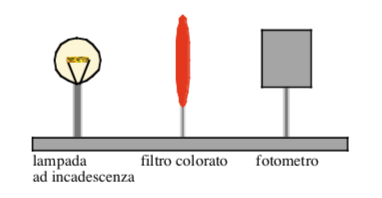
\includegraphics[width=0.3\linewidth]{figs/Setup.png}
\end{center}
La lampada ad incandescenza \`e alimentata da un generatore, con il metodo volt-amperometrico si misurano V e I.
Un fotodiodo misura l'intensit\`a luminosa emessa ad una data frequenza (selezionata da un apposito filtro inserito
tra lampadina e fotodiodo).
\vskip 0.2cm
L'intentit\`a luminosa emessa vale (legge di Planck)
\begin{align*}
   I(\nu,T) = {8\pi h \nu^3 \over c^2}\left(exp(h\nu/kT)-1 \right)^{-1}
\end{align*}
}

\frame{
  \frametitle{$h/k$ dalla misura dell'intensit\`a luminosa della lampadina}
A frequenza fissata ma a temperatura diverse (corrispondente a diverse resistenza e quindi potenze erogate
alla lampadina) si ha
\begin{align*}
   {I(T_j)\over I(T_i)} = {(exp(h\nu/kT_i)-1\over (exp(h\nu/kT_j)-1}
\end{align*}
e, siccome, a frequenze ottiche $h\nu \gg k T$ si pu\`o semplificare la relazione in
\begin{align*}
  ln\left({I_j\over I_i}\right) = {h\nu\over k} \left( {1\over T_i} - {1\over T_j} \right)
\end{align*}

Traccia dell'esperimento:
\begin{itemize}
   \item Per alcuni valori di V si misura I e la tensione del fotodiodo ($V_{fd}\propto I_{fd}$)
   \item Noto $R=V/I$ si calcola la temperatura T
   \item Si esegue un fit alla relazione di cui sopra determinando $h/k$
\end{itemize}


}

\frame
{
  \frametitle{Esperimento di Millikan (solo analisi)}

  Setup ed esempio di campione di dati (simile a quello che analizzerete)
  \begin{minipage}{0.5\linewidth}{
     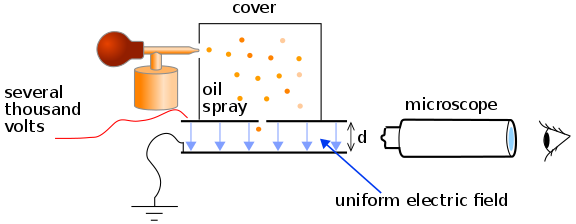
\includegraphics[width=0.9\linewidth]{figs/Mill.png}
  }\end{minipage}\begin{minipage}{0.5\linewidth}{
     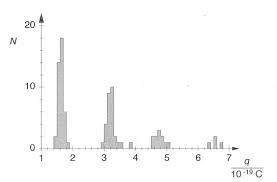
\includegraphics[width=0.9\linewidth]{figs/MillIst.png}
  }\end{minipage}
\begin{itemize}
\item Estrazione di $e$ (carica elementare) tramite fit a pi\`u gaussiane. Il valore di $e$ \`e il parametro si separazione
      tra i picchi delle gaussiane.
\end{itemize}


}
